\documentclass{article}
\usepackage[a4paper]{geometry}
\usepackage{fancyhdr} 
\usepackage{tikz}
\usepackage{amsmath}
\usepackage{hyperref} 
\pagestyle{fancy}
\lhead{Abstände zwischen Punkten und Ebenen}
\rhead{Juli 2025}
\begin{document}
   
\newcommand{\norm}[1]{\big| {#1} \big|}  
\newcommand{\vect}[1]{\overrightarrow{#1}} 
\newcommand{\vectp}[1]{\vect{\mathrm{#1}}}
  
\section{Abstände zwischen Punkten und Ebenen}
 
\begin{minipage}[t]{\dimexpr\textwidth-5cm}
 Die einfachste Methode den Abstand zwischen einem Punkt und einer Ebene zu finden, ist das \emph{Lotfußpunktverfahren}. Dabei wird ein \emph{Lotfußpunkt} $\mathrm{F}$ bestimmt, welcher der zu $\mathrm{A}$ näheste, auf $\mathrm{E}$ liegende, Punkt ist. Die Länge des Verbindungsvektors $\vectp{PF}$ stellt nun den Abstand von $\mathrm{A}$ zu $\mathrm{E}$ dar. Somit ist der Abstand
 \[
  d(\mathrm{A}, \mathrm{E}) = \norm{\vectp{PF}}
 \] 
 Weil $\mathrm{F}$ in der Regel nicht in der Aufgabe gegeben ist, muss dieser Punkt erstmal gefunden werden. Dies wird getan, indem \\[-0.7em]
\end{minipage} 
\hfill
\begin{minipage}[t]{5cm}
 \centering 
 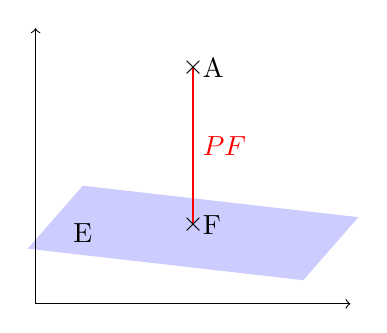
\begin{tikzpicture}[baseline=(current bounding box.north)] 
  \fill[blue!20] (-0.1, 0.7) -- (0.6, 1.5) -- (4.1,1.1) -- (3.4, 0.3) -- cycle;
  \draw (0.6, 0.9) node[black] {$\mathrm{E}$};
 
  \draw[thick,red] (2, 1) -- (2,3);
  \draw (2, 2) node[red, right] {$\vectp{PF}$}; 
  \draw (2, 3) node[black] {$\times$} node[right] {$\mathrm{A}$};  
  \draw (2, 1) node[black] {$\times$} node[right] {$\mathrm{F}$};
  \draw[->] (0, 0) -- (4, 0); 
  \draw[->] (0, 0) -- (0, 3.5);
 \end{tikzpicture}
\end{minipage}
eine Gerade, genannt die \emph{Lotgerade}, bestimmt wird, welche vom Punkt $\mathrm{A}$ aus auf direktestem Wege zur Ebene $\mathrm{E}$ geht. Offensichtlich muss die Lotgerade dafür Senkrecht zur Ebene sein, heißt kollinear zum Normalvektor $\vect{n}$. Daraus folgt die Lotgerade
\[
 g: \vect{x} = \vectp{OP} + t \cdot \vect{n} 
\]
Zusammen mit der Gleichung der Lotgerade und der Ebene kann nur deren Schnittpunkt, welcher auf der Lotfußpunkt $\mathrm{F}$ ist, gefunden werden, mithilfe dessen nun auch $\vectp{PF}$ und somit $\norm{\vectp{PF}}$ bestimmt werden kann.
 
Muss der Aufgabe nach $\mathrm{F}$ aber nicht angegeben werden, können die letzten wenigen Schritte aber auch übersprungen werden und 
\(
 d(\mathrm{A}, \mathrm{E}) = \norm{t} \cdot \norm{\vect{n}}
\)
genutzt werden. Dies folgt aus 
\begin{align*}
 d(\mathrm{A}, \mathrm{E}) &= \norm{\vectp{AF}} \\
  &= \norm{\vectp{OA} - \vectp{OF}} \\ 
  &= \norm{\vectp{OA} - (\vectp{OA} + t \cdot \vect{n})} \\
  &= \norm{t \cdot \vect{n}} \\
  &= \norm{t} \cdot \norm{\vect{n}}
\end{align*}
 
\noindent \begin{minipage}[t]{\dimexpr\textwidth-8cm} 
 \subsection{Hesse'sche Normalform}
 Hat die Ebene einen Stützpunkt $\mathrm{P}$, so kann ein rechtwinkliges Dreieck zwischen $\mathrm{P}$, $\mathrm{A}$ und einem Punkt der gleichen Distanz zwischen $\mathrm{A}$ und $\mathrm{E}$ von $\mathrm{P}$ entfernt gebildet werden. Wird in diesem Dreicken der Winkel $\alpha$ am Punkt $\mathrm{P}$ eingefügt, hat dieses die Ankathete $d(\mathrm{A}, \mathrm{E})$ und die Hypothenuse $\vectp{PA}$.
 Demnach gilt für $\alpha$
\end{minipage} 
\hfill
\begin{minipage}[t]{8cm} 
 \centering 
 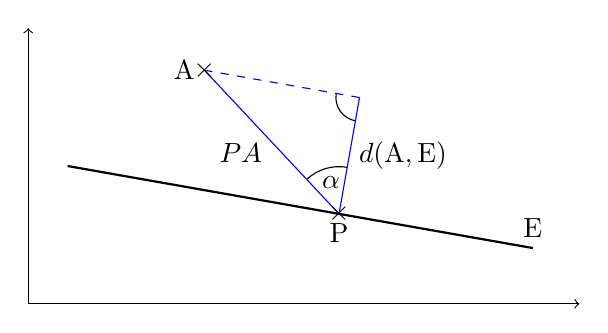
\begin{tikzpicture}[baseline=(current bounding box.north)]
  \coordinate (start) at (0.5,1.75);
  \path (start) ++({sin(100)*6}, {cos(100)*6}) coordinate (end);
  \path (start) ++({sin(100)*3.5}, {cos(100)*3.5}) coordinate (mid);
  \path (mid) ++({sin(10)*1.5}, {cos(10)*1.5}) coordinate (middist);
  \path (middist) ++({sin(-80)*2}, {cos(-80)*2}) coordinate (pointa);
  
  \draw (mid) ++({sin(10)*0.6}, {cos(10)*0.6}) arc[start angle=80, end angle=132, radius=0.6];
  \draw (middist) ++({sin(-80)*0.3}, {cos(-80)*0.3}) arc[start angle=170, end angle=260, radius=0.3];
  
  \draw[thick, black] (start) -- (end) node[above, black] {$\mathrm{E}$};
  \draw[blue] (mid) -- (middist) node[midway, right, black] {$d(\mathrm{A},\mathrm{E})$};  
  \draw[dashed, blue] (middist) -- (pointa) node[left, black] {$\mathrm{A}$};  
  \draw[blue] (mid) -- (pointa) node[midway, left, yshift=-4pt, black] {$\vectp{PA}$};
 
  \draw (mid) ++ (-0.1, 0.4) node[black] {$\alpha$};
 
  \draw (mid) node[below] {$\mathrm{P}$};  
  \draw (pointa) node {$\times$};  
  \draw (mid) node {$\times$};
 
  \draw[->] (0, 0) -- (7, 0); 
  \draw[->] (0, 0) -- (0, 3.5);
 \end{tikzpicture}   
\end{minipage} 
 
\allowdisplaybreaks 
\begin{align*} 
 cos(\alpha) &= \frac{d(\mathrm{A}, \mathrm{E})}{\norm{\vectp{PA}}}
 && \vert\, \text{Nach Distanz Umformen} \\
 d(\mathrm{A}, \mathrm{E}) &= \cos(\alpha) \cdot \norm{\vectp{PA}} 
 && \vert\, \text{\hyperref[Winkel]{$\cos(\alpha)$ durch das Skalarprodukt ausdrücken}} \\
 &= \frac{\vect{n} \cdot \vectp{PA}}{\norm{\vect{n}} \cdot \norm{\vectp{PA}}} \cdot \norm{\vectp{PA}} \\
 &= \frac{1}{\norm{\vect{n}}} \cdot \vect{n} \cdot \vectp{PA}
 && \vert\, \text{$\vectp{PA}$ in $\vectp{OA}-\vectp{OP}$ aufspalten} \\
 &= \frac{1}{\norm{\vect{n}}} \cdot \vect{n} \cdot \vectp{OA} - \vect{n} \cdot \vectp{OP}
\end{align*} 
Weil das Ergebniss bei bestimmten Winkeln negativ sein kann, welches im Kontext von Abständen aber keinen Sinn ergibt, wird die Formel in den Betrag gesetzt. Somit gilt
\[
 d(\mathrm{A}, \mathrm{E}) = \frac{1}{\norm{\vect{n}}} \cdot \norm{\vect{n} \cdot \vectp{OA} - \vect{n} \cdot \vectp{OP}} 
\] 
Offensichtlich ist ein jeder Punkt $\vect{x}$, welcher keinen Abstand zur Ebene hat, also für welchen $d(\mathrm{A}, \mathrm{E})=0$ gilt, ein Punkt auf der Ebene  
\[
 \frac{1}{|\vect{n}|} (\vect{n} \cdot \vect{x} - \vect{n} \cdot \vectp{OP}) = 0 
\] 
\end{document} 
 
 
 
 
 
